\documentclass{CUP-JNL-EDS}

%%%% Packages
\usepackage{latexsym}
\usepackage{graphicx}
\usepackage{multicol,multirow}
\usepackage{amsmath,amssymb,amsfonts}
\usepackage{accents} % load after amsmath. used for undertilde
\usepackage{bm}
\usepackage{mathrsfs}
\usepackage{amsthm}
\usepackage{rotating}
\usepackage{appendix}

%\usepackage[authoryear]{natbib}
\usepackage{biblatex}
\addbibresource{Climate_GP.bib}

\usepackage{ifpdf}
\usepackage[T1]{fontenc}
\usepackage{times}
%\usepackage{sourcesanspro}
\usepackage{newtxmath}
\usepackage{textcomp}%
\usepackage{xcolor}%
\usepackage{hyperref}
\usepackage{lipsum}
%%%%

\newcommand{\iid}{\overset{\text{i.i.d.}}{\sim}}


%\articletype{RESEARCH ARTICLE}
\jname{Environmental Data Science}
%\artid{20}
\jyear{2022}
\jvol{1}
\jissue{1}
%\jdoi{10.1017/eds.2020.xx}
%\raggedbottom


\begin{document}

\begin{Frontmatter}

\title[Article Title]{A Dependent Multi-model Approach to Climate Prediction with Gaussian Processes}

\author*[1]{Marten Thompson}\orcid{0000-0002-0012-7664}\email{thom7058@umn.edu}
\author[2]{Amy Braverman}
\author[1]{Snigdhansu Chatterjee}\orcid{0000-0002-7986-0470}

\address[1]{\orgdiv{School of Statistics}, \orgname{University of Minnesota}, \orgaddress{\city{Minneapolis}, \postcode{55455}, \state{MN},  \country{United States}}}
\address[2]{\orgdiv{Jet Propulsion Laboratory}, \orgname{California Institute of Technology}, \orgaddress{\city{Pasadena}, \postcode{91109}, \state{CA},  \country{United States}}}



\received{10 January 2022}
%\revised{01 May 2020}
%\accepted{06 May 2020}

\authormark{Marten Thompson et al.}

\keywords{Gaussian process; empirical Bayes; CMIP6}

\abstract{
Simulations of future climate contain variability arising from a number of sources, including internal stochasticity and external forcings. However, to the best of our abilities climate models and the true observed climate depend on the same underlying physical processes. In this paper we simultaneously study the outputs of multiple climate simulation models and observed data, and we seek to leverage their mean structure as well as interdependencies that may reflect the climate’s response to shared forcings.  Bayesian modeling provides a fruitful ground for the nuanced combination of multiple climate simulations. We introduce one such approach whereby a Gaussian process is used to represent a mean function common to all simulated and observed climates. Dependent random effects encode possible information contained within and between the plurality of climate model outputs and observed climate data. We propose an empirical Bayes approach to analyze such models in a computationally efficient way. This methodology is amenable to the CMIP6 model ensemble, and we demonstrate its efficacy at forecasting global average near surface air temperature. Results suggest that this model and the extensions it engenders may provide value to climate prediction and uncertainty quantification.

}

\policy{Bayesian modeling provides a fruitful ground for the nuanced combination of multiple climate model outputs when predicting the Earth's climate characteristics for the coming years. We outline one such model and describe an empirical Bayes estimation approach that is computationally efficient. The proposed methodology, when applied to CMIP6 global temperature datasets, demonstrates that using empirical Bayeisan techniques is better than using the simple ``model democracy'' approach of assigning equal weight to each climate model. We also obtain uncertainty bounds for the global temperature prediction problem.}

\end{Frontmatter}


\section[Introduction]{Introduction}

This paper is on predictive climate modeling using outputs of multiple models. The topic of how to assign weights to different climate models has been debated at length in the community. One approach is to assign equal weight to each model in multi-model climate ensembles, which has sometimes been labeled \textit{model democracy} \cite{knutti2010end}. Other approaches for using information from multiple climate models may be found in \cite{abramowitz2019esd, craigmile2017regional, knutti2017climate, sanderson2015representative, sanderson2017skill, flato2014evaluation}. Bayesian approaches with uncertainty quantification may be found in \cite{tebaldi2005quantifying, smith2009bayesian} and elsewhere. In essence, most techniques directly or implicitly balance the performance of any candidate model output on how closely it emulates current and historical data, and on how well it imitates the outputs of other climate models. Technical details on different types of multi-model ensembles, including caveats about interpreting results from such ensembles, are available in 
\cite{tebaldi2007use, knutti2010challenges, knutti2010good, knutti2013climate, knutti2010end, sunyer2014bayesian, sanderson2015addressing, knutti2017climate, sanderson2017skill, lorenz2018prospects, abramowitz2018model, herger2018selecting}, 
among other places. 
A different approach is taken in \cite{braverman2017probabilistic, chatterjee2019scale}, where models are assigned scores based on their performance in capturing probabilistic properties of observed climate data.
A review on different approaches of using climate model outputs may be found in \cite{gong2020evaluation}.

A fundamental scientific reason for studying multi-model ensembles is that the same physical processes and forces are used for all reasonable climate models, and these processes also govern the observed climate data \cite{masson2011climate}. In this paper, we leverage this property of a shared physical basis for all climate model outputs and observed data concerning global temperature data. First,  we adopt a statistical framework that assumes that the climate models' output and real data all share a common trend function over time. Second, we assume that the various model outputs and observed data are dependent on each other. This dependency is captured by framing the $L$ climate model outputs and the observed data as an $L+1$-dimensional random vector at any point in time. This allows the entire dataset in $L+1$-dimensions over time to be viewed as a \textit{vector Gaussian process}, which we discuss in some detail in Section~\ref{ss:implementation}. However, this leads to extremely challenging computations as well as a lack of transparency in the intermediate steps, hence we use an empirical Bayesian approach in this paper. 

We analyze the climate model outputs associated with the Coupled Model Intercomparison Project, now in its sixth phase (CMIP6), which directs research in fundamental areas of climate science \cite{eyring2016overview}. It organizes the federated efforts of many investigators whose model simulations examine natural climate variability and sensitivity. 
%
CMIP6 simulations occur under a wide range of scenarios %reflecting the breadth of scientific interest in climate modeling. They are 
characterized by a Shared Socioeconomic Pathway (SSP) and a level of increased radiative forcing. The Shared Socioeconomic Pathways describe a spectrum of possible futures in terms of human energy use, population, and sentiment towards climate stewardship \cite{riahi2017shared}. They then inform the quantification of land use, energy consumption, and other factors used by climate modelers. Radiative forcing concerns the increase in energy transferred through Earth's atmosphere, relative pre-Industrial levels \cite{change2007climate}. We analyze model output under SSP-5 with a radiative forcing value of 8.5 watts/m$^2$, the most aggressive increase. The SSP-5 narrative describes an increase in social and economic capital driven by fossil fuel extraction and an overall technology-driven strategy to climate change mitigation.

The focus of our analysis is the output from a selection of 17 CMIP6 simulations \cite{access-cm2,access-esm1-5,awi-cm-1-1-mr,bcc-csm2-mr,cams-csm1-0,canesm5,canesm5-canoe,fgoals-g3,giss-e2-1-g,miroc-es2l,miroc6,mpi-esm1-2-hr-DKRZ,mpi-esm1-2-lr,mri-esm2-0,noresm2-lm,noresm2-mm,ukesm1-0-ll-MOHC}. All simulations were conducted under the SSP-5 8.5 scenario and produced monthly mean global near surface air temperature values spanning 1850 January to 2100 December. We remove seasonality by subtracting the mean monthly values from 1961-1990 \cite{jones1999surface}. The observed monthly mean global near surface air temperature was also available from 1850 January to 2020 December \cite{morice2021updated}.


\section[Methods]{Methods}
\subsection{Hierarchical Bayesian Model}

The CMIP6 simulations produce monthly global near surface air temperatures from 1850-2100. Let $Y_{\ell, t}$ be the deseasonalized, mean-centered time series from $\ell$th CMIP6 climate simulation for $\ell = 1,\dots,L$. The observed monthly values through 2020 are denoted by $Y_{0,t}$. The vector $\bm{Y}_t$ will represent all values at time $t$, and $\bm{Y}_{\operatorname{cmip},t}$ will represent the $L$ climate simulations i.e.
\begin{equation}
    \bm{Y}_t = \begin{bmatrix} Y_{0,t} \\ Y_{1,t} \\ \vdots \\ Y_{L,t} \end{bmatrix}; \quad \bm{Y}_{\operatorname{cmip},t} = \begin{bmatrix}  Y_{1,t} \\ \vdots \\ Y_{L,t} \end{bmatrix}
\end{equation}

There are many ways to utilize these values when making predictions for $Y_{0,t}$. A simple method is to estimate a common mean function $\mu(t)$ shared by all the climate simulations and observed data. Here, our goal is to also leverage the information contained within the plurality of these simulations beyond their mean. One such method is to assume
\begin{align}
    \bm{Y}_t \mid \bm{U}_t &= \mu(t)\bm{1}_{L+1} + \bm{U}_t, \ \ 
    \text{ where } \ \ 
    % \label{eq:model_top}\\
    \bm{U}_t  \iid N_{L+1}(\bm{0}, \Sigma). \label{eq:mod_re}
\end{align}
where $\bm{1}_{L+1}$ is an $L+1$-dimensional vector of 1's, and $\bm{U}_t$ are independent random effects. These random elements are independent over time, but dependent between the $L+1$ time series. Our assumption here is that these are Normally distributed, but this can be relaxed.

One may wonder if assuming the $\bm{U}_{t}$ are independent over time, or identically distributed, is adequate for the available climate data. However, our extensive preliminary studies strongly indicate that there is no temporal dependency pattern in the $\bm{U}_{t}$: we have experimented using autoregressive integrated moving average (ARIMA) models, several kinds of Gaussian process-based models, conditionally heteroscedastic models and change-point detection procedures. All these preliminary studies indicate that \eqref{eq:mod_re} is the best option for modeling $\bm{U}_{t}$. However, note that our main modeling principle and ideas do not depend on the particular assumptions surrounding \eqref{eq:mod_re}. We can easily replace the Gaussian distributional assumption or the independence assumption with other suitable conditions; however in such cases even the empirical Bayesian computations would be considerably lengthier and numerical integration-driven.

We represent the common monthly mean $\mu(t)$ with a Gaussian process defined by the covariance kernel $k_{\bm{\alpha}}(\cdot, \cdot)$ parameterized by $\bm{\alpha}$. While a variety of kernels exist, the squared exponential function is a common choice. It is parameterized by $\bm{\alpha} = (\sigma^2, \gamma)$, the variance and lengthscale parameters. That is, 
\begin{align}\label{eq:mod_gp}
    \mu(t) &\sim \mathcal{GP}(0, k_{\bm{\alpha}}) \ \ \text{ where } \ \ 
    k_{\bm{\alpha}}(t_1, t_2) = \sigma^2 e^{- \gamma (t_1 - t_2)^2}.
\end{align}
Together, Equations  \ref{eq:mod_re} and \ref{eq:mod_gp} define the hierarchical model given below. 
\begin{equation}\label{eq:mod_hier}
    \begin{split}
        \bm{Y}_{t} \mid \mu(t), \Sigma &\sim N_{L+1} \left(\mu(t)\bm{1}_{L+1}, \Sigma \right),  \\
        \mu(t) & \sim \mathcal{GP}(0, k_{\bm{\alpha}}).
    \end{split}
\end{equation}


\subsection{Esimtation: Full Bayesian Approach}\label{ss:implementation}

Due to the nature of Gaussian processes, $\mu(t)$ evaluated at points $t=1,\dots,T$ will also follow a multivariate normal distribution with mean zero and a covariance matrix $K$ given by $[K]_{ij} = k_{\bm{\alpha}}(t_i, t_j)$. Thus, Equation \ref{eq:mod_hier} may alternatively be expressed as a vector Gaussian process, written here as the matrix normal distribution this induces over time $t=1,\dots,T$. Let $\undertilde{\bm{Y}}$ be the $(L+t) \times T$ matrix representing all observed and simulated time series. Let $\bm{0}_{(L+1)\times T}$ be a $(L+1)\times T$ matrix of zeros. Then,
\begin{equation}\label{eq:mod_matnorm}
\begin{split}
    \undertilde{\bm{Y}} \mid \Sigma, K &\sim MN_{(L+1), T}\big(\bm{0}_{(L+1)\times T}, \Sigma, K \big), \text{ equivalently} \\
    \operatorname{vec}(\undertilde{\bm{Y}}) \mid \Sigma, K &\sim N_{(L+1)\cdot T}\big(\bm{0}_{(L+1)\cdot T}, \Sigma \otimes K \big)
\end{split}
\end{equation}
where $\otimes$ represents the Kronecker product. 


With Equation \ref{eq:mod_matnorm}, standard properties of the multivariate Normal distribution provide pointwise predictions and uncertainty quantification via its conditional mean and conditional variance for any subset of $\operatorname{vec}(\undertilde{\bm{Y}})$. In particular, let $t_a$ corresponds to 2020 December and $t_b$ be 2100 December. The distribution of $Y_{0,t_a:t_b}$ conditional on the observed time series $Y_{0, 0:t_a}$ and CMIP6 simulations $Y_{\ell, 0:t_b}$ $\ell = 1,\dots,L$ is also multivariate normal.

Unfortunately, the matrix $\Sigma \otimes K$ is large at $(L+1)\cdot T$-dimensional square. Inverting this is cubic in complexity and infeasible for large $L$ or $T$. The manipulation of this large matrix also incurs numerical overflow issues for sufficiently large dimension.

\subsection{Estimation: Empirical Bayesian Approach}\label{ss:eb}

While the vector Gaussian process model would lend itself to full Bayesian modeling, we propose an empirical Bayesian (EB) approach. This is done in order to reduce the computational overhead and for transparency. Below we describe the method by which $\mu(t)$ and $\Sigma$ are thus estimated, and how they afford prediction and uncertainty quantification.

We estimate the common mean $\mu(t)$ as a Gaussian process on the time pointwise average of the model outputs. That is, define $\bar{Y}_{t} = 1/(L+1) \sum_{\ell = 0}^{L} Y_{\ell, t}$.
%\begin{align*} 
%\bar{Y}_{t} = \frac{1}{L+1} \sum_{\ell = 0}^{L} Y_{\ell, t}. 
%\end{align*}
Then, the parameters $\bm{\alpha}=(\sigma^2, \gamma)$ are estimated by maximizing the marginal likelihood of $\Bar{Y}_{t}$ under the Gaussian process model. Denote the estimated values of the mean function at time $t$ as $\hat{\mu}(t)$.

Next, take $\hat{U}_{\ell,t} = Y_{\ell,t} - \hat{\mu}(t)$. Then, let $\hat{\bm{U}}_t = [ \hat{U}_{0,t} \; \hat{U}_{1,t} \dots \hat{U}_{L,t}]^\top $.
%\begin{equation*}
%    \hat{\bm{U}}_t = \begin{bmatrix} \hat{U}_{0,t} \\ \hat{U}_{1,t} \\ \vdots \\ \hat{U}_{L,t} \end{bmatrix}
%\end{equation*}
Use $\hat{\bm{U}}_1,\dots,\hat{\bm{U}}_T$ to get $\hat{\Sigma}$, the $(L+1) \times (L +1)$ variance-covariance matrix. This encodes the possible correlations between time series outside of the common mean, most importantly between the observed time series and the CMIP6 simulations' outputs. Let us write 
\begin{align} \label{eq:sigma_hat}
    \hat{\Sigma} = \left(   \begin{array}{ll} 
    \hat{\sigma}_{0}^{2} & \hat{\Sigma}_{0}^{T} \\
    \hat{\Sigma}_{0} & \hat{\Sigma}_{\operatorname{cmip}} \\
    \end{array}
    \right)
\end{align}
where $\hat{\sigma}_{0}^{2}$ is the variance of the observed data's random effects, and $\hat{\Sigma}_{\operatorname{cmip}}$ is the $L \times L$ covariance between random effects associated with the CMIP6 outputs.

One of our goals is to predict $Y_{0, t}$ for $t \in $ 2021-2100 given the model outputs and historic observations. The distribution of these values follows from Equation $\ref{eq:mod_hier}$ and standard properties of the Normal distribution. Given $\hat{\mu}(t)$ and simulated values $\bm{Y}_{\operatorname{cmip},t}$% = \bm{y}_{\operatorname{cmip},t}$ 
% \vspace*{-0.9cm}
\begin{align}
        Y_{0,t} \mid  \hat{\mu}(t), \bm{Y}_{\operatorname{cmip},t} &\sim N(m^*, \gamma^*) \label{eq:cond_pred_y} \\
        m^* &=  \hat{\mu}(t) + \Sigma_{0}^{T} \Sigma_{\operatorname{cmip}}^{-1} \bigl( \bm{Y}_{\operatorname{cmip}, t} - \hat{\mu}(t)\bm{1}_L \bigr) \label{eq:cond_pred_mean}\\
        \gamma^* &= \sigma_{0}^{2} - \Sigma_{0}^{T} \Sigma_{\operatorname{cmip}}^{-1}\Sigma_{0} \label{eq:cond_pred_cov}
\end{align}
These conditional mean and variance values provide natural point estimates and uncertainty quantification. Note that using $\hat{\mu}(t)$ alone amounts to making predictions with the unconditional mean. In the next section, we will see that the conditional mean better reflects the month-to-month variation of these time series, as well as differences between them and the common mean.


\section[Results]{CMIP6 Results}

\subsection{Leave-One-Out Validation}\label{ss:loo_comp}
A leave-one-out (LOO) style of evaluation allows us to investigate the validity of this approach. Setting aside the observed time series $Y_{0,t}$, the remaining CMIP6 simulations all span 1850 January to 2100 December. One by one, each of the available time series is singled out and treated like the ``observed'' values. That is, it is truncated to 2020 November, and we perform the model estimation approach from Section \ref{ss:eb}. This produces predictions through 2100, which we compare to the full time series's actual values. 

As a tangible example, Figure \ref{fig:loo_acess-cm2} depicts the results when the access-cm2 CMIP6 simulation is being treated like the observed time series. Predictions begin in 2020 December and continue to 2100 December. They match the actual simulated values both in broad trend across the whole of their domain, and in local month-to-month fluctuations. Note also that while the common mean function $\hat{\mu}(t)$ trends below the simulated values as time continues, the conditional mean (Equation \ref{eq:cond_pred_mean}) ameliorates this trend.

\begin{figure}[h]
    \centering
    \begin{tabular}{c c}
        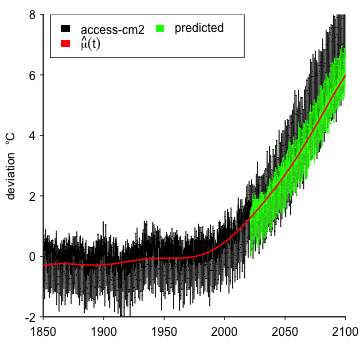
\includegraphics[width=0.4\textwidth]{paper/figs/loo_access-cm2.png} 
        &  
        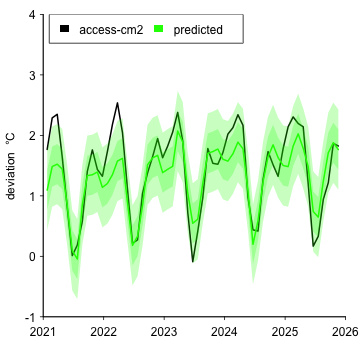
\includegraphics[width=0.4\textwidth]{paper/figs/zoomloo_access-cm2.png} \\
        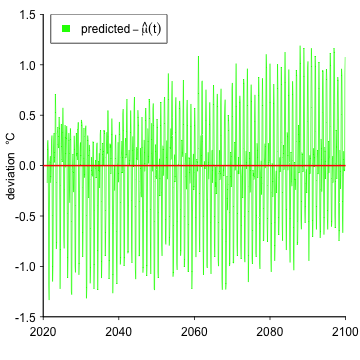
\includegraphics[width=0.4\textwidth]{paper/figs/condeff_access-cm2.png} & 
    \end{tabular}
    \caption{Amongst others, we used the access-cm2 CMIP6 time series to evaluate our model's predictive accuracy. The top left figure shows the whole of the training and test intervals, 1850 January - 2020 November and 2020 December - 2100 December, respectively. Just five years are shown in the top right figure, starting in 2021 January, to highlight the prediction's month-to-month accuracy. Light and dark shading indicate one and two standard deviations from the conditional mean, as found in Equations \ref{eq:cond_pred_mean} and \ref{eq:cond_pred_cov}. On the top and bottom left we see the conditional mean also improves predictions by inducing a trend that better matches that of the test interval compared to $\hat{\mu}(t)$}
    \label{fig:loo_acess-cm2}
\end{figure}

Table \ref{tab:loo_mse} contains a summary of the LOO results. It includes the mean squared error between the actual output of the indicated simulation and the predictions of our empirical Bayes (EB) model. Compare these to the MSE of the predictions found using just the common mean function $\hat{\mu}(t)$ or pointwise average $\Bar{Y}_t$. The empirical Bayes model is more performant than the common mean in every case.
\vspace{-0.2cm}
\begin{table}[h]
\small
    \centering
    \begin{tabular}{l | c c c}
     LOO Sim &  MSE$_{\operatorname{EB}}$ & MSE$_{\hat{\mu}}$ & MSE$_{\Bar{Y}_{t}}$ \\
     \hline
    access-cm2      & 0.44 & 1.01 & 0.38 \\
    access-esm1-5   & 0.16 & 0.41 & 0.09 \\
    bcc-csm2-mr     & 0.43 & 0.64 & 0.42 \\
    canesm5-canoe   & 3.57 & 4.09 & 3.72 \\
    canesm5         & 3.40 & 3.97 & 3.58 \\ 
    cesm2-waccm     & 0.59 & 1.03 & 0.58 \\
    cesm2           & 0.49 & 0.89 & 0.47 \\
    giss-e2-1-g     & 0.57 & 0.73 & 0.64 \\
    mcm-ua-1-0      & 0.39 & 0.72 & 0.64 \\
    miroc-es2l      & 0.64 & 1.06 & 0.66 \\
    miroc6          & 0.84 & 1.48 & 0.97 \\
    mpi-esm1-2-hr   & 0.83 & 1.08 & 0.98 \\
    mpi-esm1-2-lr   & 0.83 & 0.95 & 0.87 \\
    mri-esm2-0      & 0.34 & 0.69 & 0.26 \\
    noresm2-lm      & 1.30 & 1.68 & 1.29 \\
    noresm2-mm      & 1.12 & 1.45 & 1.20 \\
    ukesm1-0-ll     & 3.22 & 3.79 & 3.24 
    \end{tabular}
    \caption{Each CMIP6 simulation was treated like the observed time series, truncated to 2020 November, and predicted by various methods. The predictions produced by our empirical Bayes model are similar in accuracy to using $\bar{Y}_{t}$ itself and also provide an estimate of variability. These predictions were superior to the common mean component $\hat{\mu}(t)$ on every CMIP6 test simulation.}
    \label{tab:loo_mse}
\end{table}



\subsection{Observed Time Series}
Making predictions for the observed climate follows the procedure outlined in Section \ref{ss:eb}. Figure \ref{fig:observed_pred} depicts the predicted values for the observed time series $Y_{0,t}$ from 2020 December - 2100 December. The upward trend is driven by the common mean $\hat{\mu}(t)$ estimated on the CMIP6 time series. The random effects induce the month-to-month variations, shown in Subsection \ref{ss:loo_comp} to better reflect CMIP6 time series. 

Note that the observed time series has less variation than the CMIP6 simulations considered here. Over the shared period of 1850 January to 2020 November, the observed time series has variance 0.15 compared to 0.55 for the CMIP6 simulations on average. Comparing Figure \ref{fig:observed_pred} to the access-cm2 data in Figure \ref{fig:loo_acess-cm2} is representative of this. This is then reflected in the covariance matrix Equation \ref{eq:sigma_hat}; its attenuating presence in Equation \ref{eq:cond_pred_mean} explains how the predictions in Figure \ref{fig:observed_pred} show less variation than those in Figure \ref{fig:loo_acess-cm2}.

\begin{figure}[h]
    \centering
    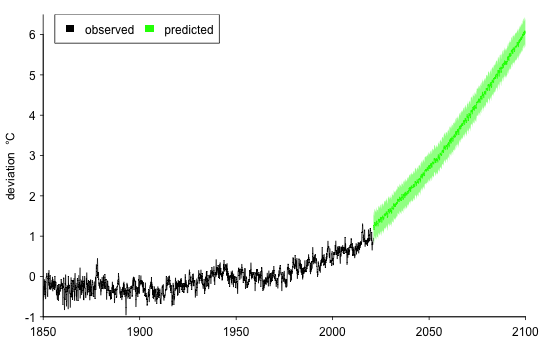
\includegraphics[width=0.65\textwidth]{paper/figs/observed_pred_nomuhat.png}
    \caption{Predicted values for mean global surface temperature using Equation~\ref{eq:cond_pred_mean}, with shading to $\pm 2$ standard deviations (Equation~\ref{eq:cond_pred_cov}). This model leverages the common mean as well as individual correlations amongst CMIP6 simulations and historical observed data}
    \label{fig:observed_pred}
\end{figure}


\section{Conclusion}
This preliminary investigation affirms the use of our hierarchical Bayesian model in combining multi-model climate data. Our model reflects both the small and large scale deviational properties of a given time series vis a vis a common mean. An empirical Bayesian treatment is an attractive approach to estimating this model; additional climate simulations can be considered with little added computational cost. This is especially important in applications where simulations produce high-dimensional output as is common in climate science.

%\section{Future work}
Our model assumes that the properties of the common trend $\mu (\cdot)$ can be adequately captured using a Gaussian process. This can be easily extended to a $t$-process or an elliptically contoured process with some additional computations. Also, our model  extends to the case where there is a spatial component in the data or where we consider regional climate models: the principles outlines above extend simply to such cases.

% \bibliographystyle{plain}
%\bibliography{Climate_GP}


\begin{Backmatter}

%\paragraph{Acknowledgments}
%We are grateful for the technical assistance of A. Author.

\paragraph{Funding Statement}
This research is partially  supported by
the US National Science Foundation (NSF) under grants 
 1939916, 1939956, and a grant from Cisco Systems Inc.


\paragraph{Competing Interests}
The authors declare none.

\paragraph{Data Availability Statement}
All materials and code necessary to reproduce these results may be found at \url{https://github.com/MartenThompson/climate_informatics_2022}. Please see relevant citations for CMIP6 \cite{access-cm2,access-esm1-5,awi-cm-1-1-mr,bcc-csm2-mr,cams-csm1-0,canesm5,canesm5-canoe,fgoals-g3,giss-e2-1-g,miroc-es2l,miroc6,mpi-esm1-2-hr-DKRZ,mpi-esm1-2-lr,mri-esm2-0,noresm2-lm,noresm2-mm,ukesm1-0-ll-MOHC}  and observed data \cite{jones1999surface, morice2021updated}. 


\paragraph{Ethical Standards}
The research meets all ethical guidelines, including adherence to the legal requirements of the study country.

\paragraph{Author Contributions}
\textbf{Marten Thompson}: Conceptualization, Methodology, Formal analysis, Software, Writing - Original Draft. 
\textbf{Amy Braverman}: Data Curation, Supervision.
\textbf{Snigdhansu Chatterjee}: Conceptualization, Methodology, Supervision, Writing - Review \& Editing. 


\paragraph{Supplementary Material} None.
%State whether any supplementary material intended for publication has been provided with the submission.

\printbibliography

\end{Backmatter}


\end{document}
